\documentclass[a4paper,twocolumn]{esapub2005} % European paper
\pagestyle{empty}

% introduce this option for the ESA publications style
\bibliographystyle{alpha}

\usepackage{graphicx,subfigure} %for figures \usepackage{subfig} %forsubfigures
\usepackage[fleqn]{amsmath}    % need for subequations
\usepackage{multirow} % for complex tables \usepackage{multicol} % for columnsspliting
\usepackage{color} %for highlight text \usepackage{booktabs}
\usepackage{url}
\usepackage{units}
\usepackage{floatrow}
\usepackage{float}

\graphicspath{{img/}}
\restylefloat{table}

\title{First Experimental Investigations on Wheel Walking for Improving
Triple-Bogie Rover Locomotion Performances}

\author[1]{Martin Azkarate}
\author[1]{Martin Zwick}
\author[2]{Javier Hidalgo-Carrio}
\author[1]{Robin Nelen}
\author[3]{Tim Wiese}
\author[1]{Pantelis Poulakis}
\author[1]{Luc Joudrier}
\author[1]{Gianfranco Visentin}
\affil[1]{European Space Agency, ESA, Noordwijk, The Netherlands}
\affil[2]{Robotics Innovation Center, DFKI, Bremen, Germany}
\affil[3]{Technische Universit\"at M\"unchen, TUM, Munich, Germany}


\newcommand{\btx}{\textsc{Bib}\TeX} \newcommand{\filename}{esapub}

\begin{document}

\keywords{\LaTeX; ESA; macros}

\maketitle

\section*{Abstract}

\textbf{On November 2014 a test campaign was carried out in the Automation and
Robotics Laboratory of ESTEC to evaluate the performance of Wheel Walking
manoeuvres in different scenarios. This paper shows the experimental results
obtained during the campaign and the performance analysis made when comparing
wheel walking with standard rolling.}

\section{Introduction}

Planetary rover missions to Mars such as NASA's MER or MSL have shown a clear
decrease of the traversing capabilities while rolling across some particular
surface areas of Mars. Loose soil and fine dust terrain is the scenario where
rovers may experience the most significant loss of their tractive performance.
The extreme of these cases was encountered in the Spirit rover which got
permanently stuck on May 2009 while traversing the loose sandy area of Troy
~\cite{SpiritTrap}.

Previous studies at JPL ~\cite{ROB:ROB21481} introduce the concept of the
Effective Ground Pressure (EGP) as a first order of approximation for an
inversely proportional indicator of the traversing capabilities of a rover. In
relation to this, ExoMars' estimated EGP (considering an effectively larger
wheel due to its flexible properties) is about 2.5 times the one of MER and
MSL.

Deployment actuators of a triple-bogie rover locomotion platform could in
principle be used to perform wheel-walking manoeuvres.  How wheel walking could
affect the traversing capabilities of rovers when driving on the aforementioned
disadvantageous terrain types is a recurrent debate in the planetary robotics
community. The Russians Lunokhod and Marsokhod rovers already used in the past
a locomotion concept named peristaltic motion very similar to the wheel walking
concept explained in this paper  with which they claimed to gain "amazing
slope climbing and obstacle overcoming capabilities" ~\cite{Ehrenfreund1998}.

This led the Automation \& Robotics Lab of ESTEC to initiate an internal
project aiming at the development of wheel-walking control algorithms and the
assessment of the subsequent locomotion performances. The target platform of
this investigation is a triple-bogie laboratory prototype, namely ExoTeR.

This paper briefly presents the ExoTeR rover in section 2, the wheel-walking
concept in triple-bogie locomotion configurations in section 3 and focuses in
section 4 on the first experimental results obtained for three different
operational scenarios, comparing key performance metrics between the wheel
walking and rolling locomotion modes. The three operational scenarios
considered are: 1) entrapment in loose sand, 2) up-slope traverse and 3) rover
egress. Section 5 gives the conclusions drawn from these experiments and in
section 6 the future work and test plan is explained.

\section{The ExoMars Testing Rover}

The rover platform used for the experiments described hereafter is an
ExoMars-like scaled down version laboratory prototype. The ExoMars Testing
Rover (ExoTeR)~\cite{Azkarate2015} mimics the locomotion configuration of
ExoMars (according to its design in 2007/8), a.k.a. triple bogie passive
suspension, with a parallelogram structure on top of each bogie. The locomotion
subsystem comprises 6 wheels and 16 actuated joints, more precisely, 6 driving,
4 steering and 6 deployment –or walking– motors.  Motion control electronics
are a network of servo-drives, namely Elmo Whistles, connected in a CAN Bus
together with the on-board computer. A driver module in the OBC acts as a CAN
Master implementing the CANOpen protocol and sends joint commands timely
synchronised to perform a certain locomotion manoeuvre. Each servo-drive takes
care of the close-loop control of one active joint to reach the commanded
(position and/or velocity) set point.  Figure 1 illustrates the locomotion
system of ExoTeR. Inside the uncovered body the motion control electronics can
also be seen.

\begin{figure}[h!]
    \centering
    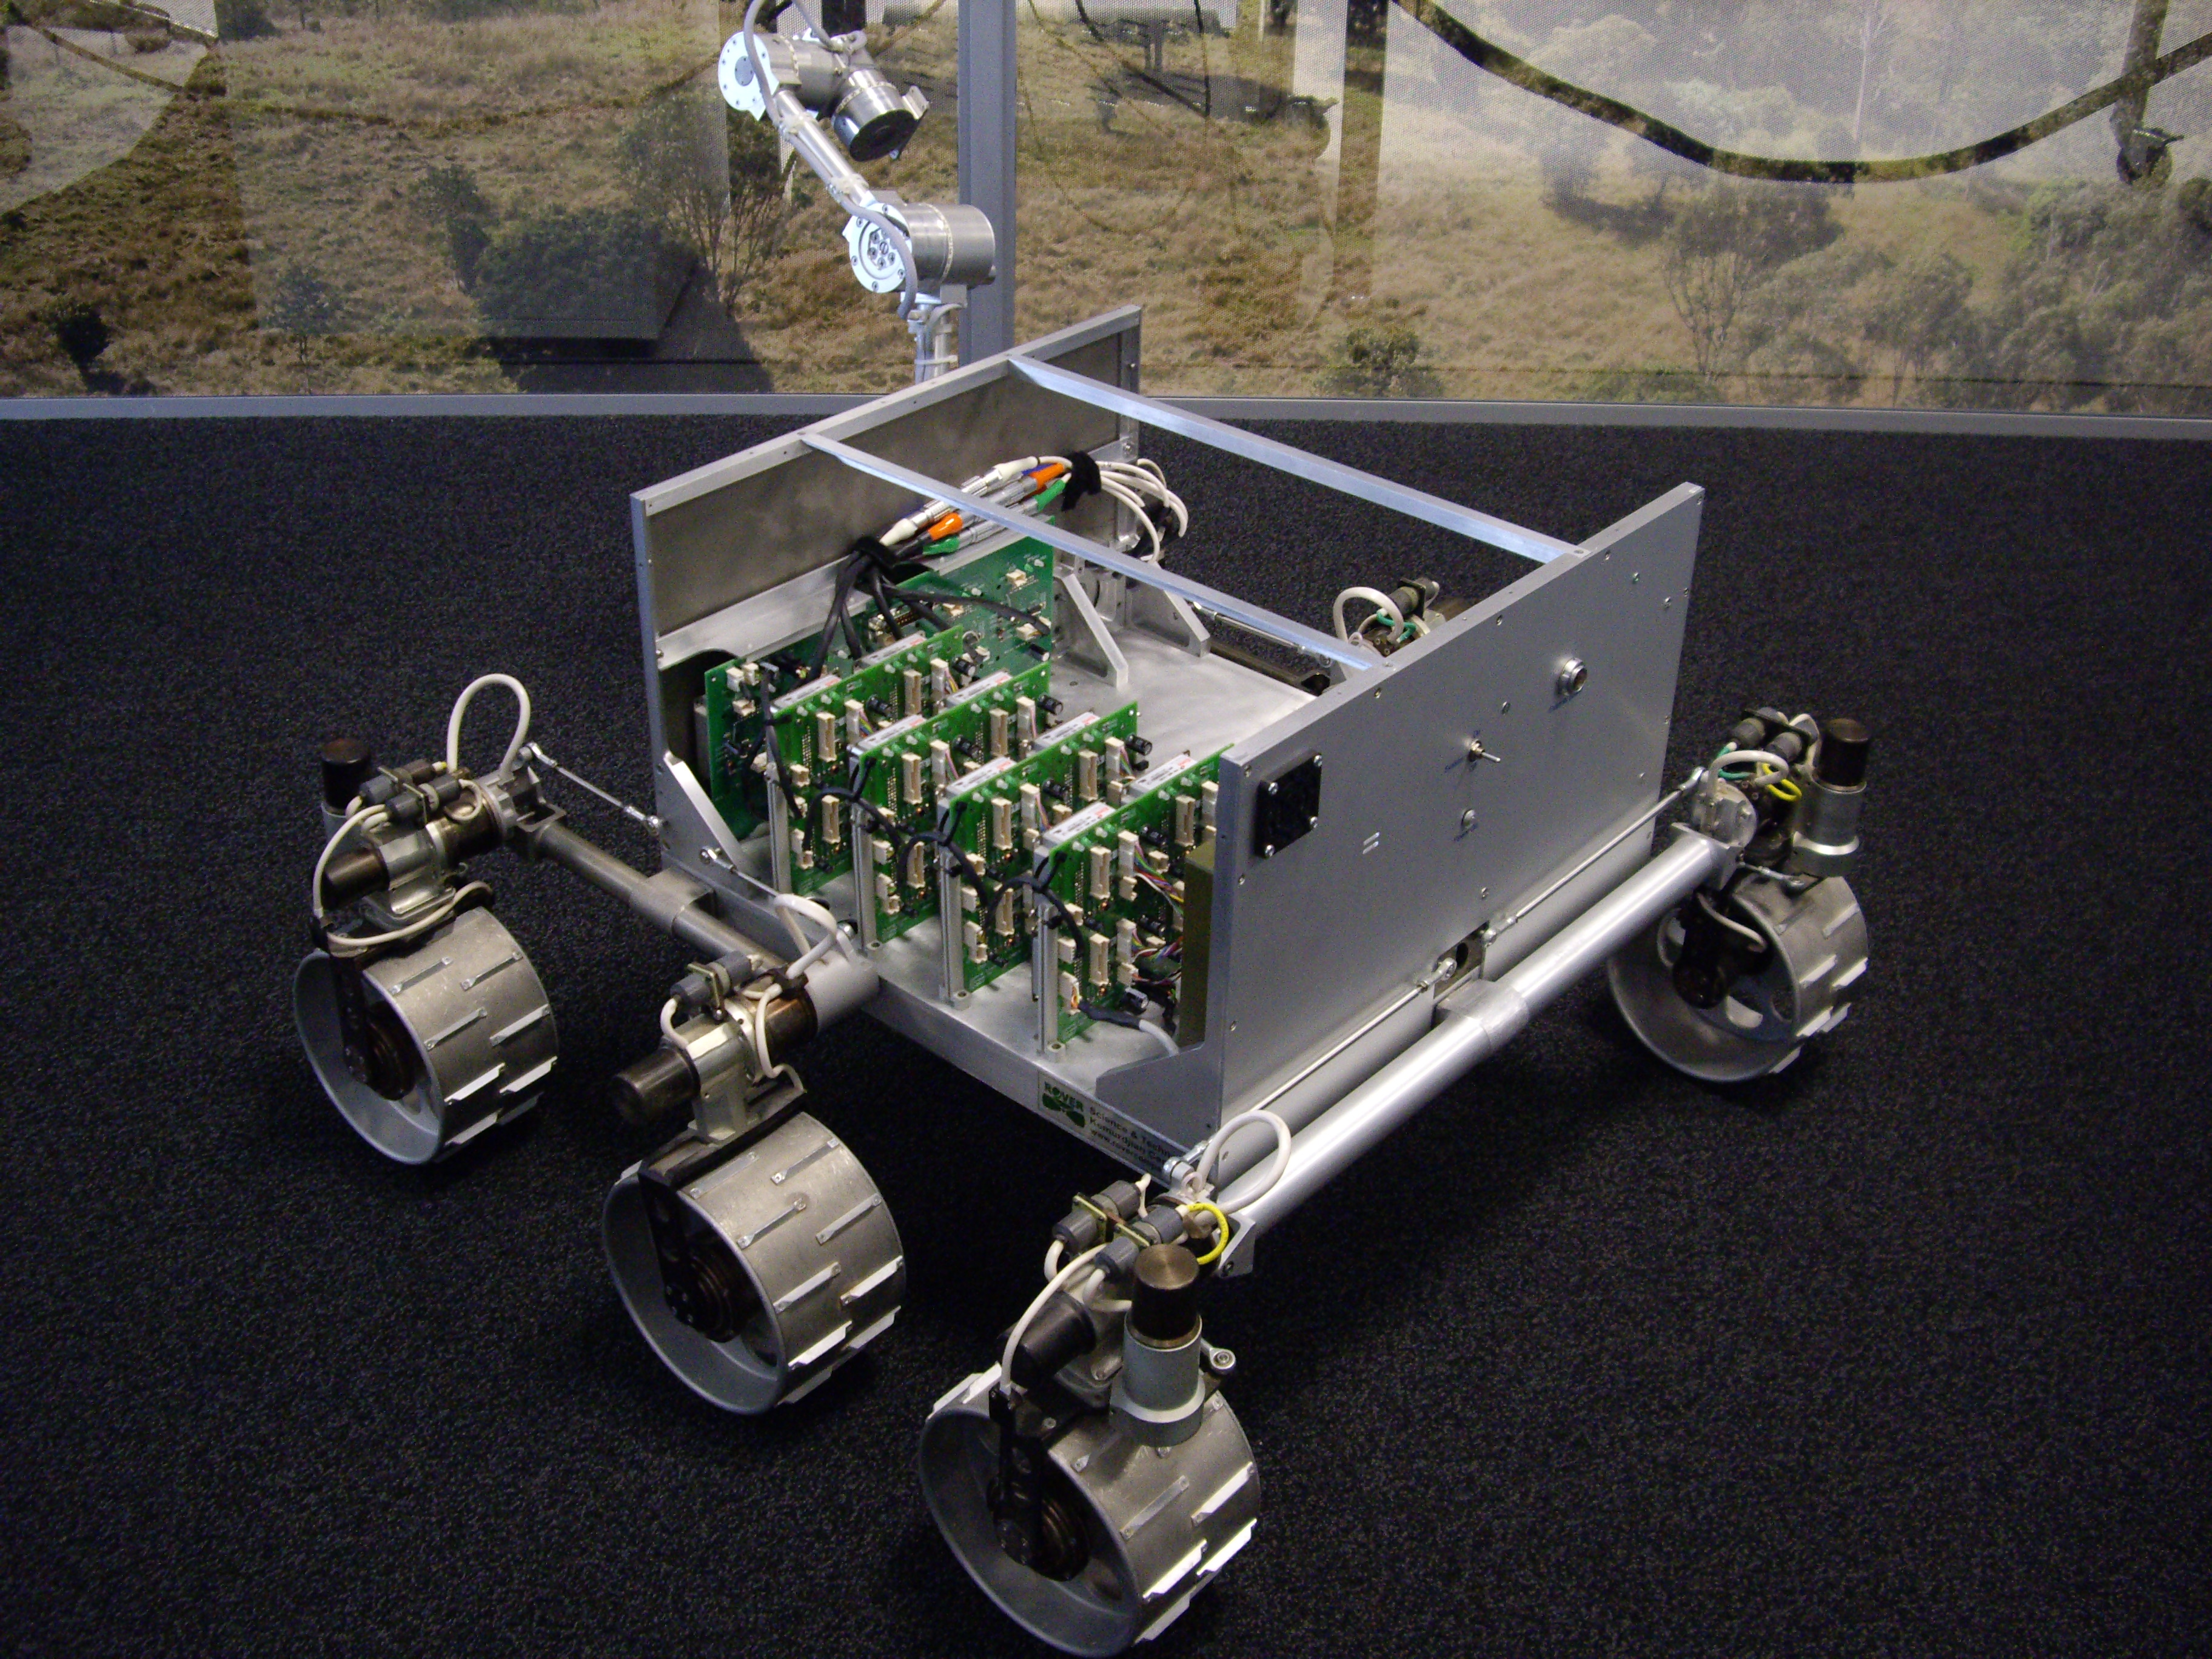
\includegraphics[width=0.9\textwidth]{ExoterRover2013.jpg}
    \caption{ExoTeR Rover, 2013}
    \label{fig:volley}
\end{figure}

The platform dimensions are approximately $70~\times~70$~\unit{cm} in foot
print and 40~\unit{cm} high.  The wheels are 14~\unit{cm} in diameter and
9~\unit{cm} in width, which together with its total mass of 23.92~\unit{kg}
are equivalent to an EGP of 6.21~\unit{kPa}. The rover system currently
includes a mast structure and PTU mechanism with mechanical interfaces to
attach a stereo camera and a ToF camera as well. Other sensors include an
Inertial Measurement Unit, and incremental encoders and absolute position
sensors for the active and passive joints of the locomotion kinematic chain.
The system is used to perform R\&D activities in the fields of: system
integration, locomotion performance, control architecture design and
implementation, and sensor data fusion among others. 

\section{Wheel Walking Implementation}

Global body commands of motion are commonly performed using a motion model.
Kinematics motion models have real-time capabilities and are inexpensive in
comparison with sophisticated wheel-dynamic simulation techniques.  The
wheel-walking evaluation presented in this paper uses a method which is able to
\textit{optimally}\footnotemark[2] combine the motion induced at each contact
point. The primary contribution of the model is fusing, in a unified framework,
desired body velocities to joint motion commands as a whole.  The
implementation of a complete motion model behaves more consistent and stable
than previous wheel walking techniques. The model makes use of the
transformation approach~\cite{Tarokh2005} to accurately model 6-DoF kinematics.
It derives from the work in~\cite{Hidalgo-Carrio2014} to invert the Jacobian
formula from the odometry kinematics.

The model requires a minimum of two coordinate frames per kinematic chain: a
robot body frame ($B$) attached to the desired rover center and a contact frame
($C_{il}$) defined as a single point of contact between the robot and the
ground. Those coordinate frames are related to each other by means of the
Jacobian matrix in the velocity domain. The matrix maps Cartesian to joint
velocities and relates the rover pose rates to joints and sensed rate
quantities as:

\begin{equation}
    \left[\dot{x}_{B} ~ \dot{y}_{B} ~ \dot{z}_{B} ~ \dot{\phi}_{B}
    ~ \dot{\theta}_{B} ~ \dot{\psi}_{B} ~ \right]^T = J_{il}
    \left[\boldsymbol{\dot{q}} ~ \boldsymbol{\dot{\varepsilon}}_{il} \right]^T
    \label{eq:wheeljacobian}
\end{equation}

where $\boldsymbol{\dot{q}}$ are the desire joint rates to command to the
actuators.  Different wheel walking gaits (i.e. motion patterns) are set by
dynamically setting constraints in the Jacobian. Each Jacobian defines the
contribution of each kinematic chain to the body motion allowing the analysis
of each chain and contact point to the resulting final velocity in the robot
body.  Considering a single contact angle $\dot{\varepsilon}_{il}$ the $J_{il}$
matrix size is $6 \times (n + 6)$ where $n$ corresponds to the DoF of the
mechanism.  The composite rover equations are obtained combining the Jacobian
matrices for all kinematic chains into a sparse matrix equation of appropriate
dimensions. The desired solution is obtained by numerically solving a system of
equations using Weighted Least-Squares.


\footnotetext[2]{Optimally here refers to the best estimated value from a
weighted least-squares perspective.}

\section{Experimental results}

Three different scenarios are considered to evaluate the traversability
performance of the wheel walking locomotion mechanisms, each of them referring
to situations where the rover could potentially benefit from the wheel walking
actuation.

\subsection{Loose sand} This test is supposed to simulate a trapped situation
from which the rover should free itself. It is the first wheel walking
performance test executed with ExoTeR. The baseline of the test is to verify
the operative readiness of the implemented wheel walking algorithms in a load
wise representative environment.

\subsubsection{Setup} The test facility is improvised in an outdoor volleyball
court on a sunny day (see picture \ref{fig:volley}). The sandy part the rover
is driving on has no overall slope. The soil is a normal beach volleyball
silica sand with a mixed grain size of 0.063 - 2.0~\unit{mm}. Due to previous rainfall
some days before, the soil is slightly moist and develops cohesive properties
as seen in picture \ref{fig:volleyexoterdigg}. The sand gets equally prepared
with a raking procedure into approximately 10~\unit{cm} depth before each run.  The
rover is commanded wireless and runs on battery. No ground truth system is used
in this experiment. 
%The rover was tested on a quartz sand with quartz gravel similar to the
%outdoor beach volleyball sand. The objective of the test was to verify the
%operative readiness of the implemented WheelWalking algorithms in a load wise
%representative environment. Picture \ref{fig:volley} shows the used setup. It
%consists of the ESTEC beach volleyball court, a bench, a camera, a power
%supply, a generator (not in the picture) and a ground control station (not in
%the picture).

%Soil BeachVolleyball: Silica sand [dry and moist], grainsize:0.063 - 2 mm ,
%wet/moist => cohesive soil

\begin{figure}[h!]
    \centering
    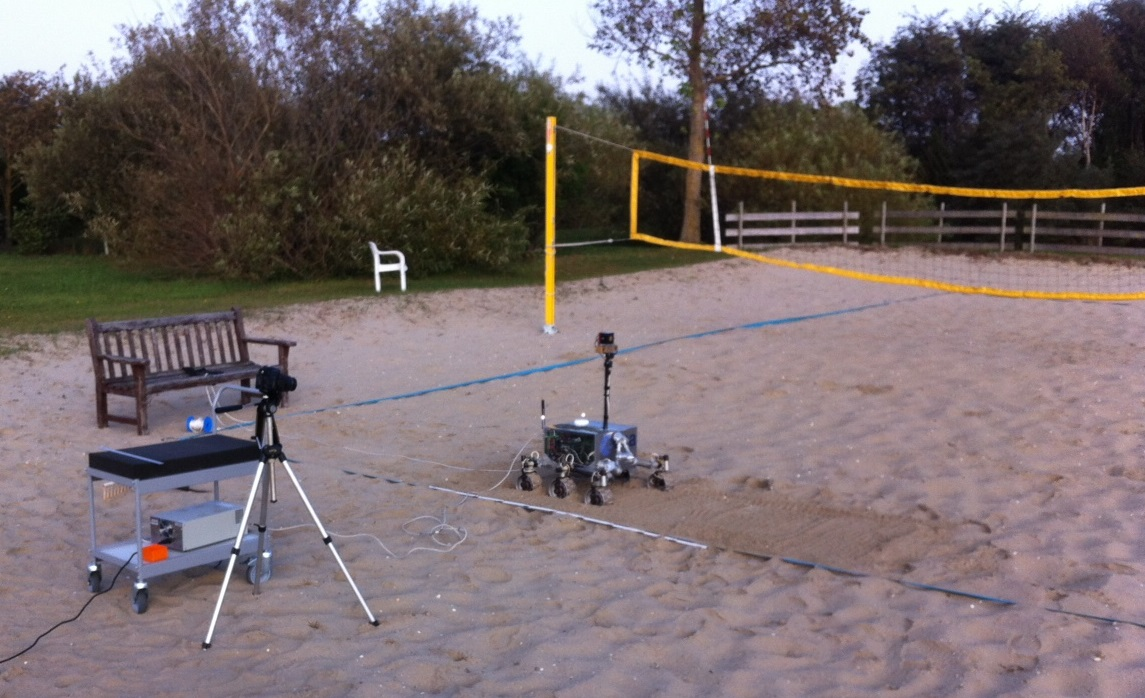
\includegraphics[width=0.9\textwidth]{volley.jpg}
    \caption{Setup on outdoor beach volleyball court}
    \label{fig:volley}
\end{figure}

\subsubsection{Test procedure}

The used procedure is divided in two characteristic parts. The first part is to
get the rover stuck in a repeatable way. Therefore the rear bogie is tied to
the bench with a detachable rope. With the rope on tension, the rover starts
driving away from the bench. Once the drawbar pull and the tension have the
same value, the rover does not produce any forward motion anymore and keeps
digging itself into the ground as shown in Figure \ref{fig:volleyexoterdigg}.
This stops once the rear wheels are sunk by half their diameter into the soil.
After that, the rope gets untied and part two starts. The system restarts in
normal driving or wheel walking mode and the data starts recording. 

\begin{figure}[h!]
    \centering
    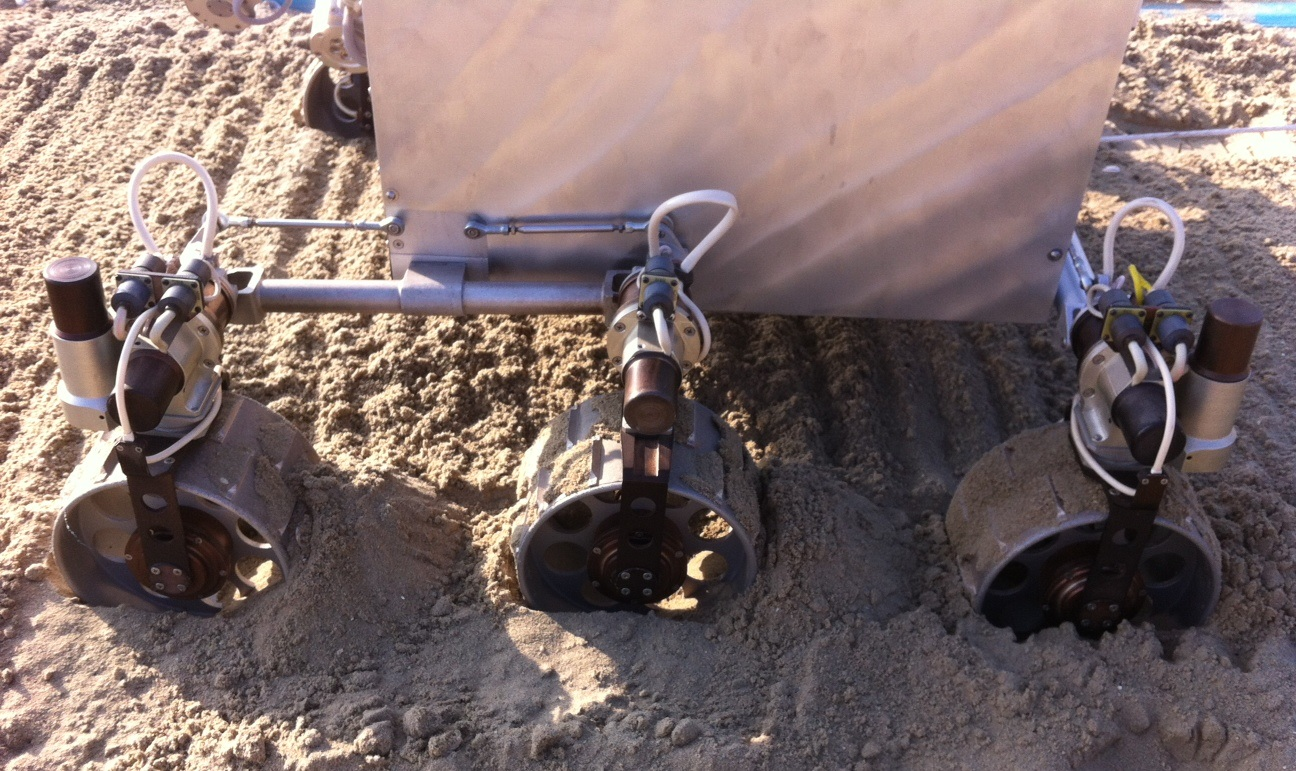
\includegraphics[width=0.9\textwidth]{volleyexoterdigg.jpg}
    \caption{ExoTeR bogged down by half a wheel diameter}
    \label{fig:volleyexoterdigg}
\end{figure}

\subsubsection{Tests} The two modes that are compared are normal driving versus
the [Side-by-Side] wheel walking gait. Both are commanded at a 2 $\frac{cm}{s}$
body velocity. 

\begin{figure}[h!]
    \centering	
    \subfigure{
        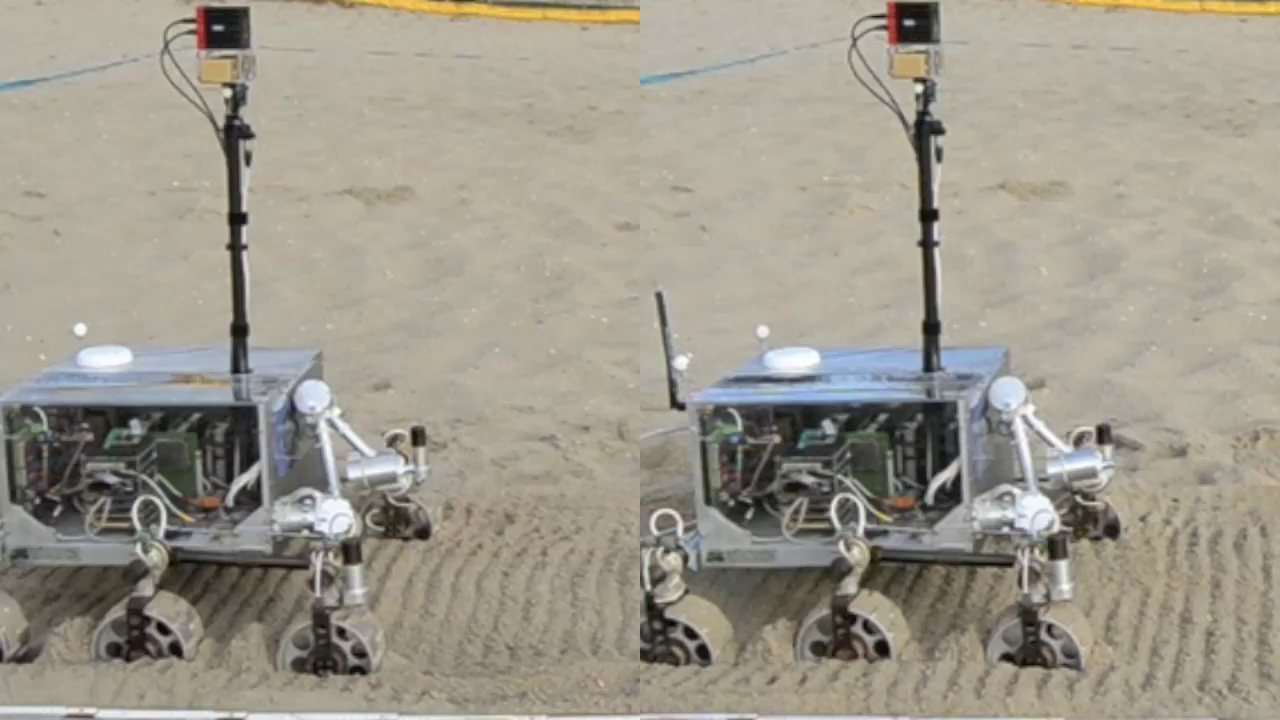
\includegraphics[width=0.45\textwidth]{volleystuck00.png}
        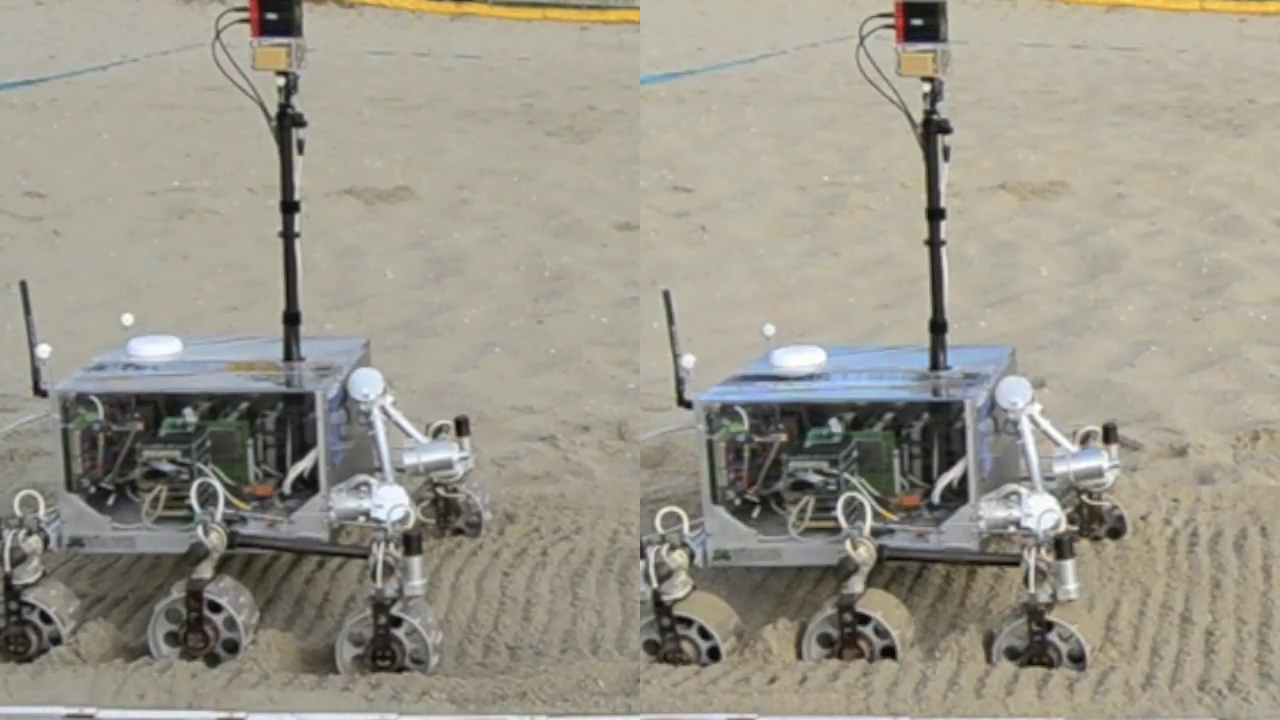
\includegraphics[width=0.45\textwidth]{volleystuck15.png}
    }	
    \subfigure{
        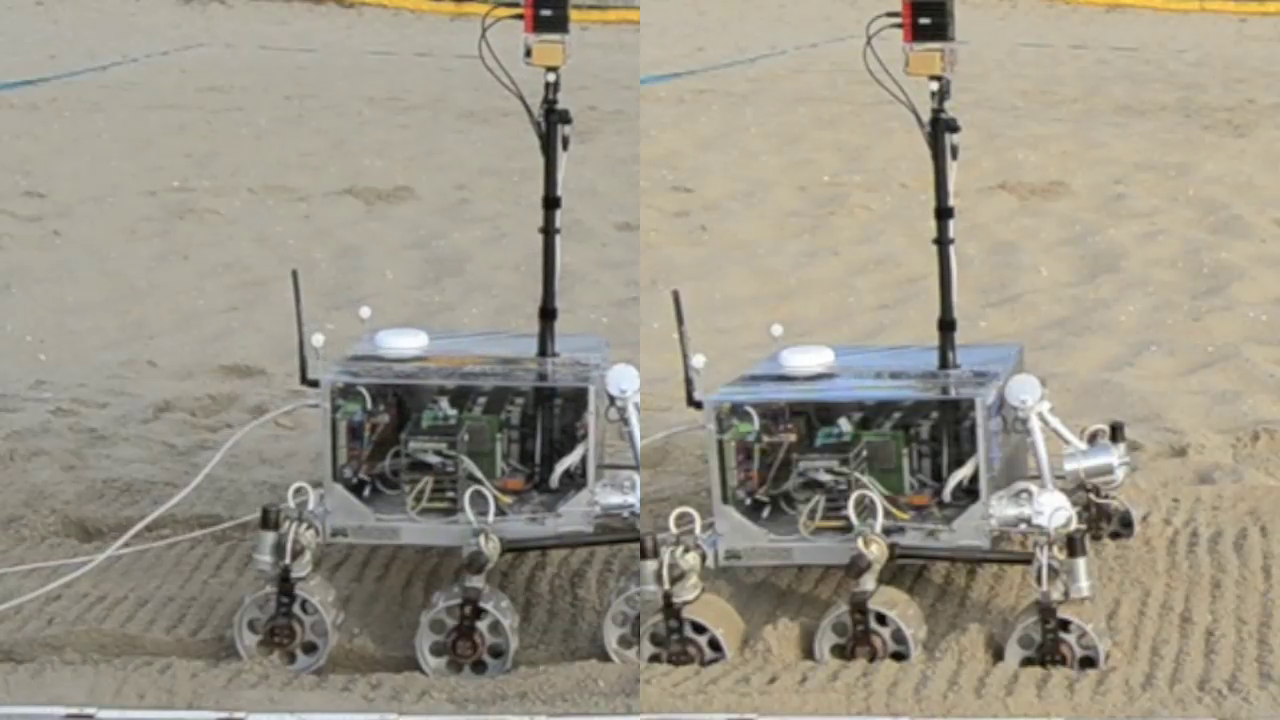
\includegraphics[width=0.45\textwidth]{volleystuck30.png}
        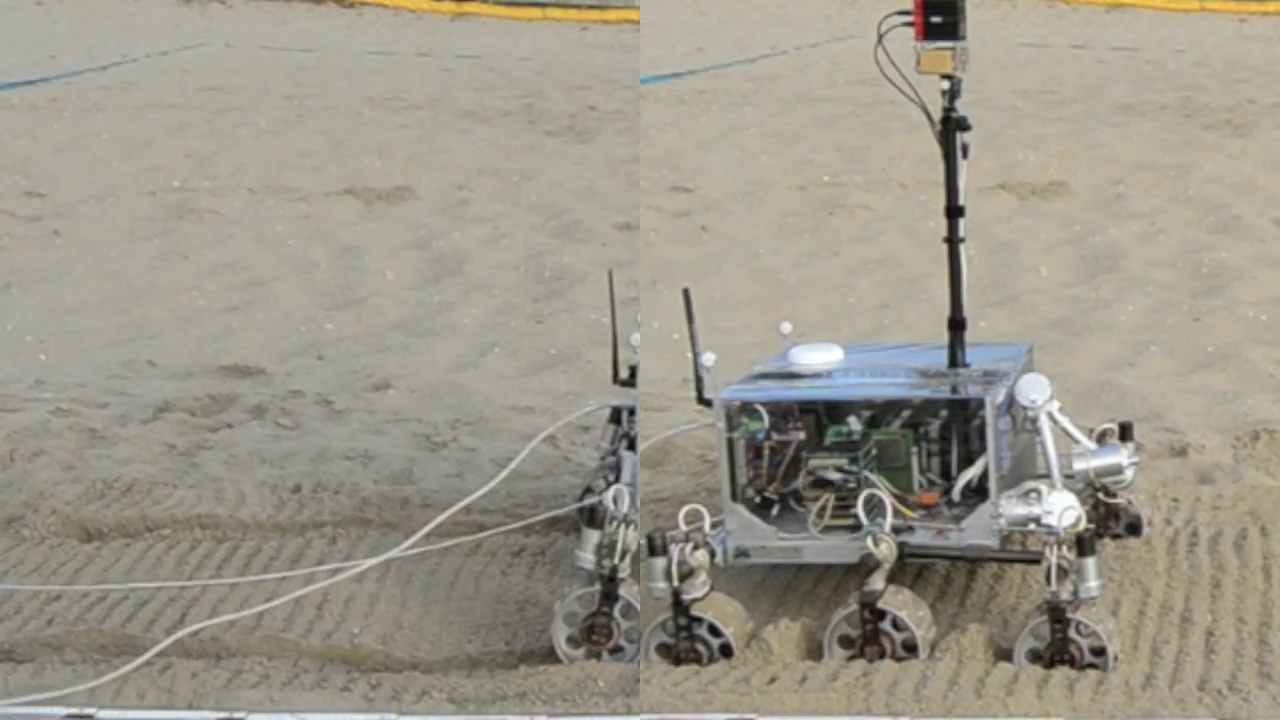
\includegraphics[width=0.45\textwidth]{volleystuck45.png} }
        \caption{top-left:t=0s,  top-right:t=15s, bottom-left:t=30s,
        bottom-right:t=45s; each picture has wheel walking on the left half and
        normal driving on its right half }
    \label{fig:volleysequence}
\end{figure}

The photo array in figure \ref{fig:volleysequence} shows the progress of the
two modes, normal driving and wheel walking while trying to set the rover free.
The result is a tremendous benefit of wheel walking. After 45 seconds, normal
driving reaches 3~\unit{cm} and thereby averages a 97\% slip ratio. The wheel walking
run is completely freed after 20 seconds. Assuming that under normal
circumstances, the rover gets trapped while normal driving, it would be even
more unlikely that it would be able to free itself without wheel walking.

%The metric for this test had a binary format. On the one hand, the rover
%failed to get out of the stuck ( $ > 99 \% $  slip ratio) situation using
%standard driving actuation. On the other hand, using wheel walking locomotion
%in approx. 20 seconds the rover was able to overcome the situation and achieve
%to perform at commanded rover body velocity ( $ < 10 \% $ slip ratio).

%================================================================
%================================================================
\subsection{Slope Tests}

Areas with high inclination are particularly interested to test wheel-walking
capabilities. This section describes the experimental setup and results in detail.

\subsubsection{Setup} The objective of the experiments is to test the wheel
walking capability on slopes. The rover has to drive from the bottom to the top
of the slope in two modes and successfully repeat this three times per mode.
First the rover performs the traverse three times in normal driving mode
followed by three tests in wheel walking mode. The tests are done on
0$^{\circ}$, 10$^{\circ}$, 15$^{\circ}$ \& 20$^{\circ}$ slope angles. 

\paragraph{Soil characteristics and environment} The different slope angles are
realized with a soil filled one axis automotive trailer (see photo
\ref{fig:trailer}). It's pivot is the single axis which allows an inclination
form approximately -10$^{\circ}$ up to +25$^{\circ}$. Due to the limited
bearing capacity of the trailer, only a 2~\unit{m} $\times$ 1.1~\unit{m}
$\times$ 0.25~\unit{m} (length $\times$ width $\times$ depth) is filled with
soil. Cardboard boxes fill the leftover volume. In this setup, the filling
depth is more than twice the wheel diameter and the distance to any walls
during a test run is high enough to assume  the boundary effects to be
negligible.  The used soil is 80\% ES3-OMR from Sibelco Ltd mixed with 20\%
gravel provided my KIBAG Zentrallabor. The gravel has a grain size distribution
of 16\% 0-4~\unit{mm}, 18\% 4-8~\unit{mm}, 15\% 8-11~\unit{mm}, 21\%
11-16~\unit{mm} and 30\% 16-22~\unit{mm}.  A 100 Hz Vicon tracking system is
used for the ground truth and orientation. The ES3 itself simulates a coarse
sandy to gravelly material occurring in scree, polymodal surficial lags and
local coarser aeolian accumulations. The coarse scree and aeolian accumulations
can occur in terrain with rocky escarpments \cite{michaud2014}.


%Soil ES3-OMR with gravel: Full description of this soil: OMR DRY (from Sibelco
%Ltd, United Kingdom) 80% by mass, with uniformly admixed Hart-splitt gravel,
%16% 0-4 mm, 18% 4-8 mm, 15 % 8-11 mm, 21% 11-16 mm, 30 % 16-22 mm (from KIBAG
%Zentrallabor, Switzerland).

 %ES3 is a coarse sandy to gravelly material occurring in scree, polymodal
%surficial lags and local coarser aeolian accumulations. The coarse scree and
%aeolian accumulations can occur in terrain with rocky escarpments [MI14].


\begin{figure}[h!]
    \centering
    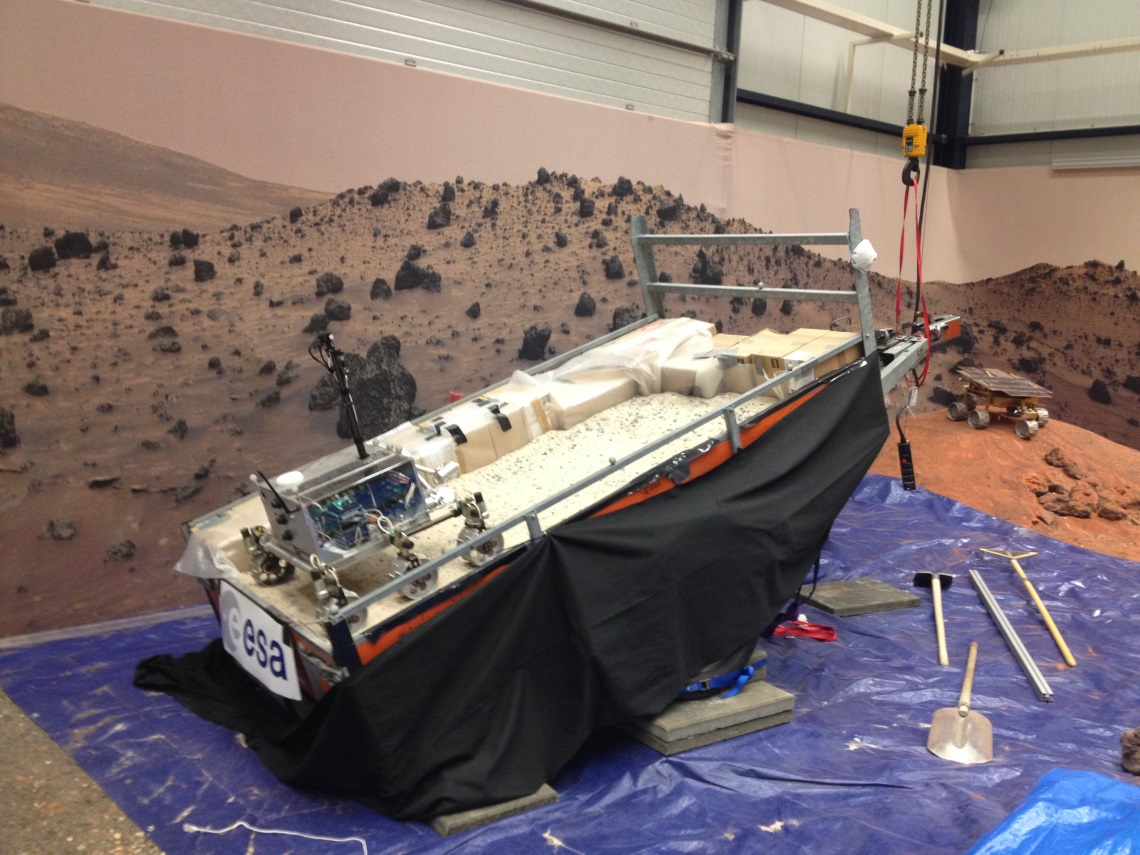
\includegraphics[width=0.9\textwidth]{trailersetup.jpg}
    \caption{Trailer in ESTEC's Mars terrain}
    \label{fig:trailer}
\end{figure}
%_____________________________________________________________


\subsubsection{Test procedure}
%placing, soil preparation, gaits, number of repeatings, abort cirieria, 



\begin{figure}[h!]
    \centering
    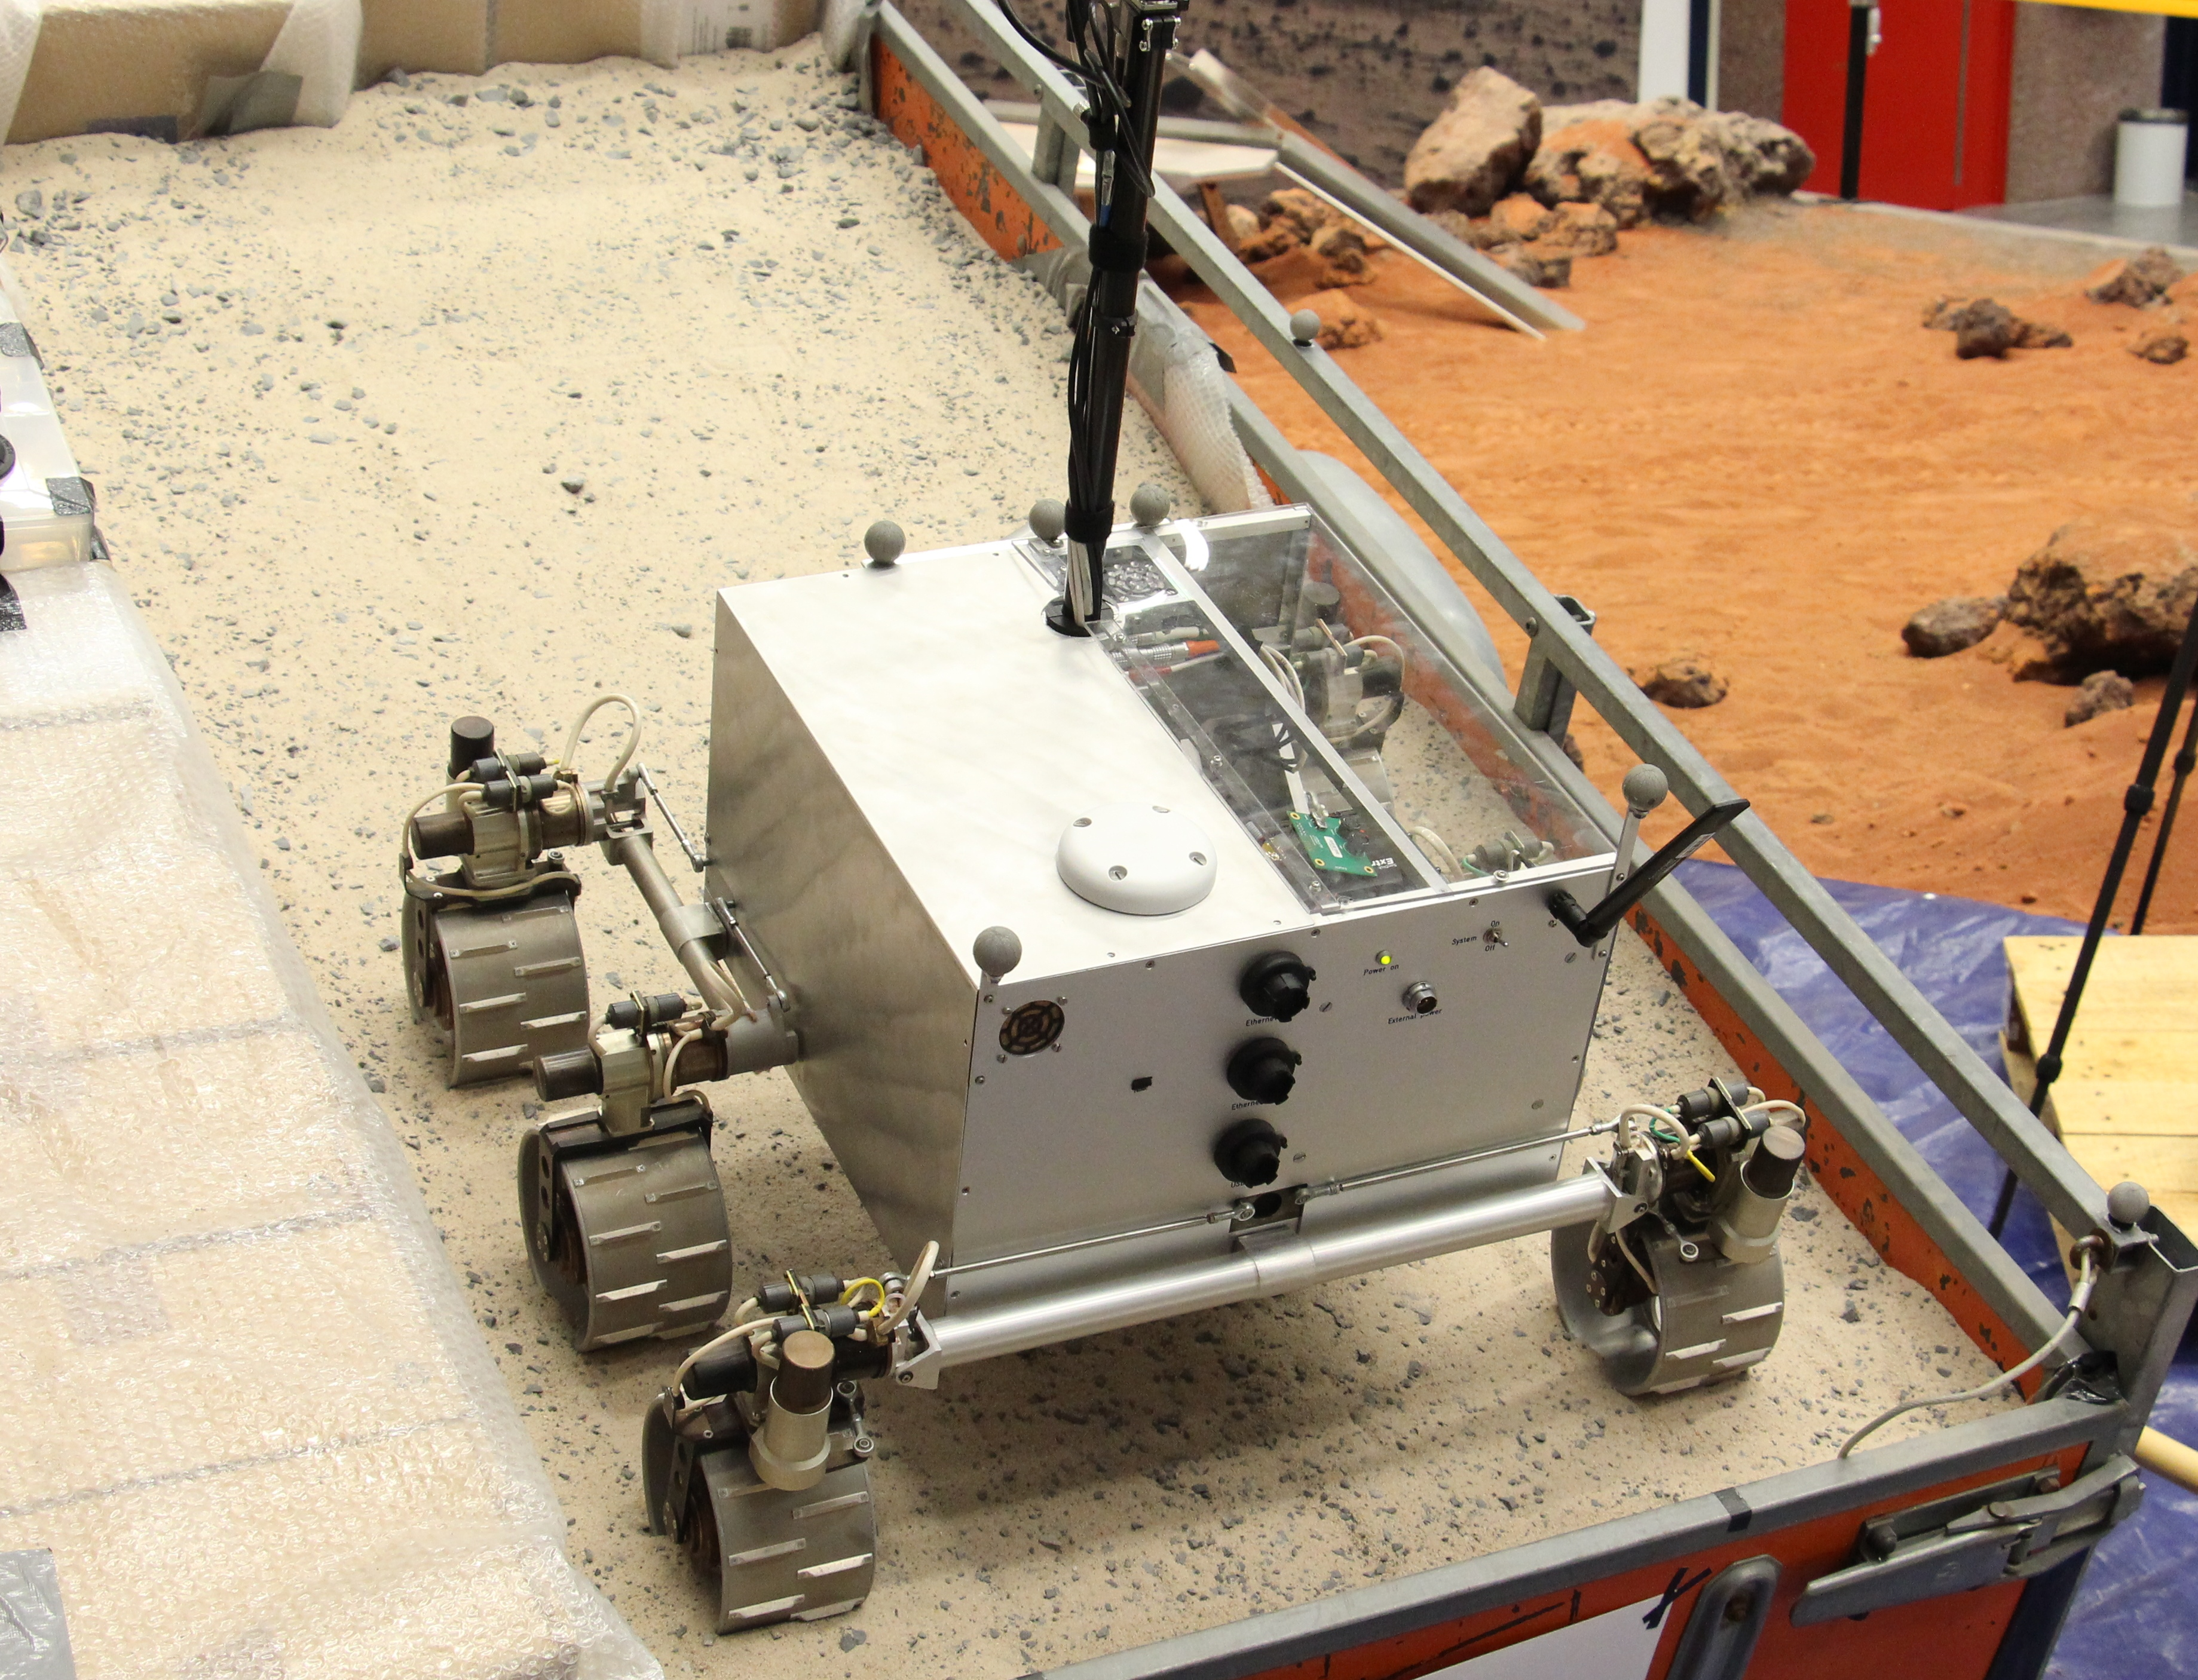
\includegraphics[width=0.9\textwidth]{Exoslope.jpg}
    \caption{ExoTeR rover on 15$^{\circ}$ slope in the trailer}
    \label{fig:Exoslope}
\end{figure}

\subsubsection{Tests} For further comparison purpose the unit of slip-ratio is
used as shown in formula \ref{eq:slip}.

\begin{equation} slip = 1- \frac{real\, position\, tracked\, by\,
cameras}{position\, estimated\, by\, wheel\, odometry} \label{eq:slip}
\end{equation}

Prior to the here analysed tests, there have been qualification runs on a
17.5$^{\circ}$ slope to define the superior gait.  The side-by-side gait
performed best in terms of slip and heading stability and was therefore chosen. 

%Other gaits were also used on the dry run tests and after the plan for slope
%tests had been completed. All other tested gaits (AXLE_BY_AXLE and EVEN_ODD or
%TRIPOD) showed to have worse performance in the preliminary tests, i.e. higher
%slip ratios. 

The following plots (\ref{fig:00d}, \ref{fig:10d}, \ref{fig:15d} \&
\ref{fig:20d}) show the resulting slip ratios obtained in each of the slope
angles for standard driving and wheel walking. All off them show three valid
wheel walking tests and three normal driving tests. These sets are always shown
in the same coloring. The blue lines represent the slip of the three normal
driving tests on a scale from 0 to 1. The red ones do the same for the wheel
walking tests. The distance the normal driving accomplished in respect to the
time are represented in green. Cyan shows the distance over time for the wheel
walking ones.

In the 0$^\circ$ run (Figure \ref{fig:00d}) the different driving modes have
barely any performance difference even though all WW lines show a slightly
better performance in the slip plots. But this difference is negligible for
such low slip values. Both plot groups show a small peek in the first 10
seconds in which the rover develops a little sinkage and goes into steady
state. 


\begin{figure}[h!]
    \centering
    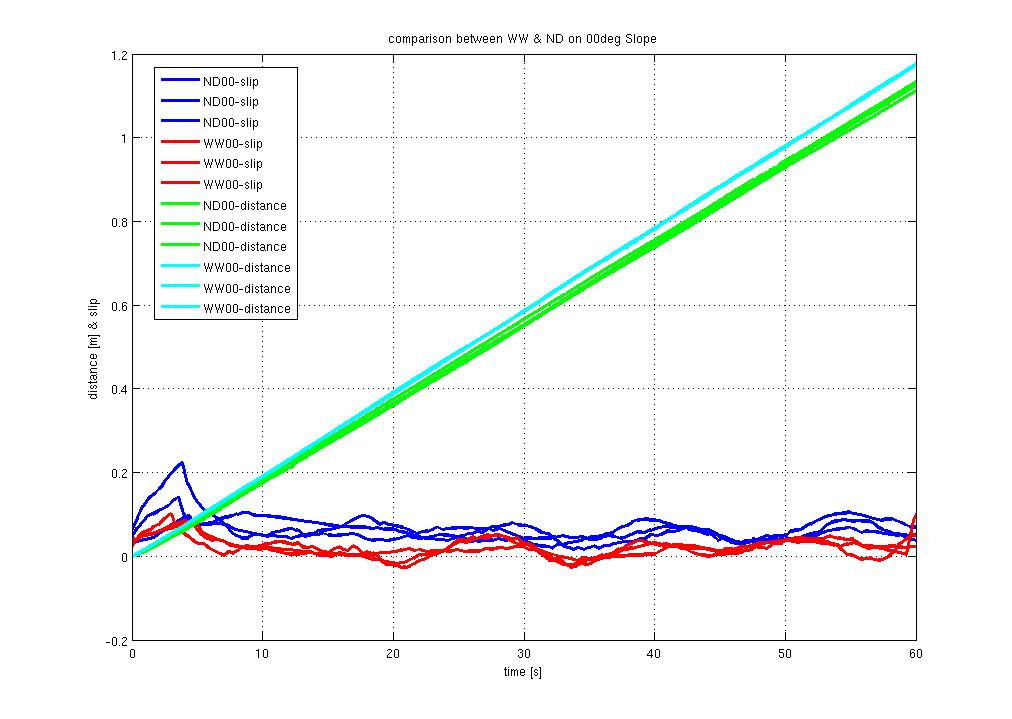
\includegraphics[width=0.9\textwidth]{00d.jpg}
    \caption{Comparison between wheel walking and normal driving on flat terrain}
    \label{fig:00d}
\end{figure}

The performance difference in the 10$^\circ$ slope already show the benefit of
wheel walking compared to normal driving. The slip value of former is about
50\% less than in the later case. Still, the slip for both is considered low.
At 15$^\circ$ slope however (Figure \ref{fig:15d}), the difference gets way
more visible in terms of traversed distance.  Figure \ref{fig:20d} with its
20$^\circ$ slope shows the biggest performance difference. The travelled
distance is roughly double in case of wheel walking, what means that it has
half the average slip. The average slip for wheel walking for the three runs
was 82.4\% compared to 89.2\% in the normal driving (averaged in steady state
from t=75~\unit{s} - t=250~\unit{s}).  The small periodic ripples in the wheel
walking runs are generated by the walking motion. While having slip ratios
above approximately 10\%, the rover starts waving around a point in between the
two rear axels which is not the rover origin. Therefore the tracking shows
ripples with a frequency of about 0.7~\unit{Hz}

\begin{figure}[h!]
    \centering
    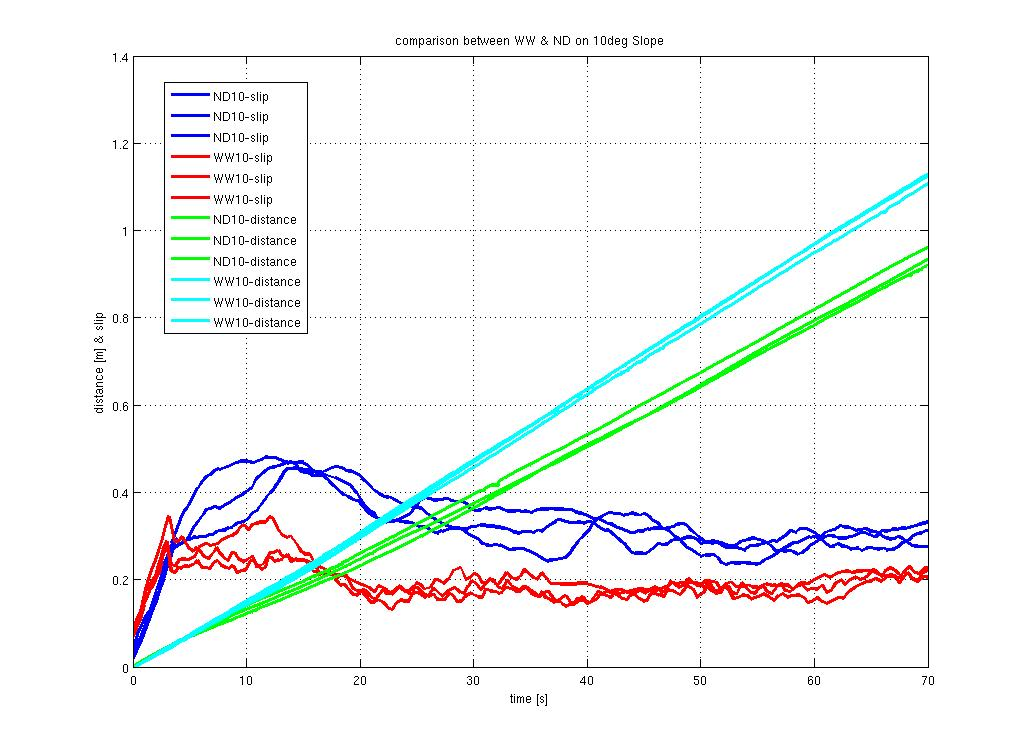
\includegraphics[width=0.9\textwidth]{10d.jpg}	\caption{Comparison between
    wheel walking and normal driving on a 10$^{\circ}$ Slope} \label{fig:10d}
\end{figure}

\begin{figure}[h!]
    \centering
    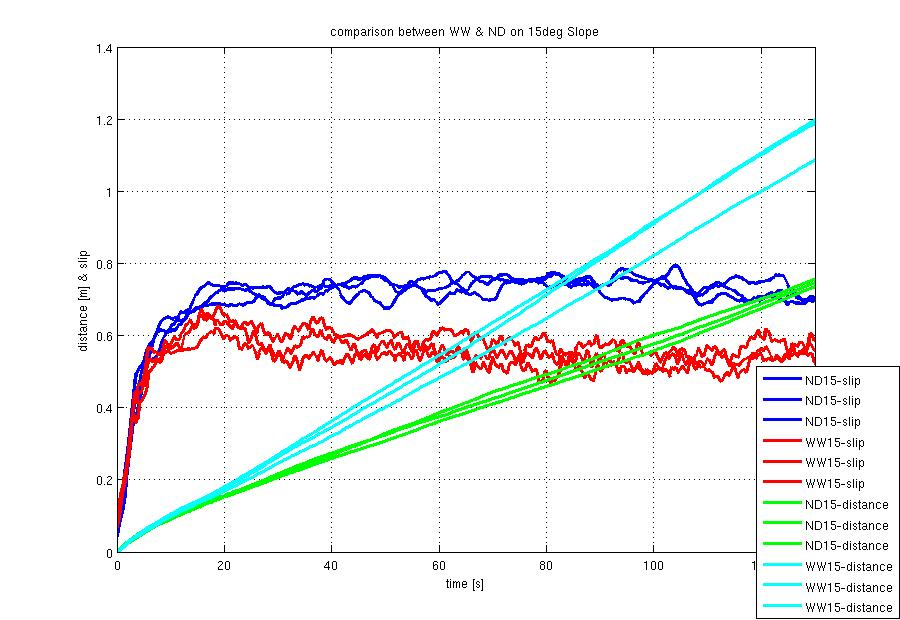
\includegraphics[width=0.9\textwidth]{15d.jpg}	\caption{Comparison between
    wheel walking and normal driving on a 15$^{\circ}$ Slope} \label{fig:15d}
\end{figure}

\begin{figure}[h!]
    \centering
    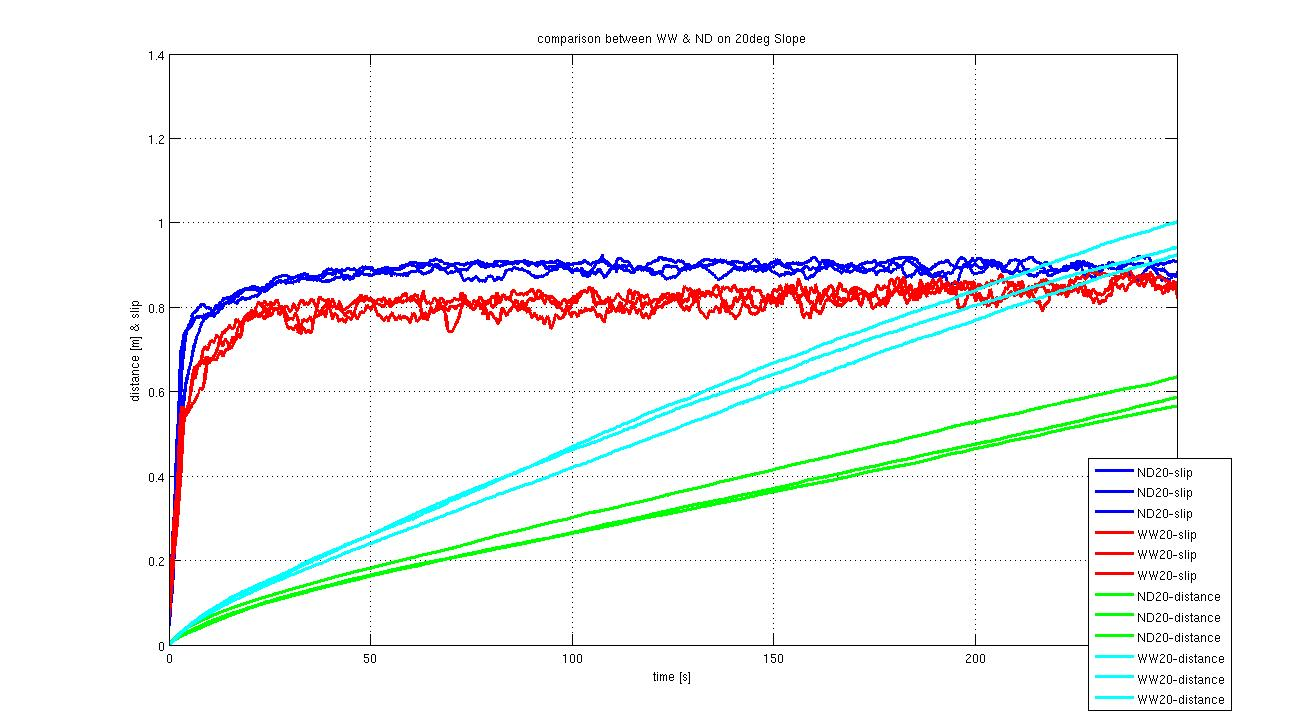
\includegraphics[width=0.9\textwidth]{20d.jpg}	\caption{Comparison between
    wheel walking and normal driving on a 20$^{\circ}$ Slope} \label{fig:20d}
\end{figure}



A series of tests at 20$^{\circ}$ slope angle were run changing the step length
at each run, from 2.5~\unit{cm} to 12.5~\unit{cm} incrementing the step length by 2.5 cm at
each test. The results of these series of tests are inconclusive so far, as no
specific relation can be identified between the step length and the slip ratio.

Other experimental tests include running the system backwards and/or fixing the
walking motors to the position equal to the angular value of the slope. This is
supposed to reduce the load in the back wheels of the rover by shifting the CoM
forward and therefore distribute the weight equally over the three axis and
hence increase in theory the traversability performance. The plot (figure
\ref{fig:ndr20d}) shows the slip ratios obtained for the case of running
backwards with the walking actuators angled in position compared to normal
driving forwards. The driving backwards means that the two bogies are in the
back and make an equal load on all four wheels of these bogies due to ExoTeR's
parallel mechanisms.  These measures do not show any benefit.


\begin{figure}[h!]
    \centering
    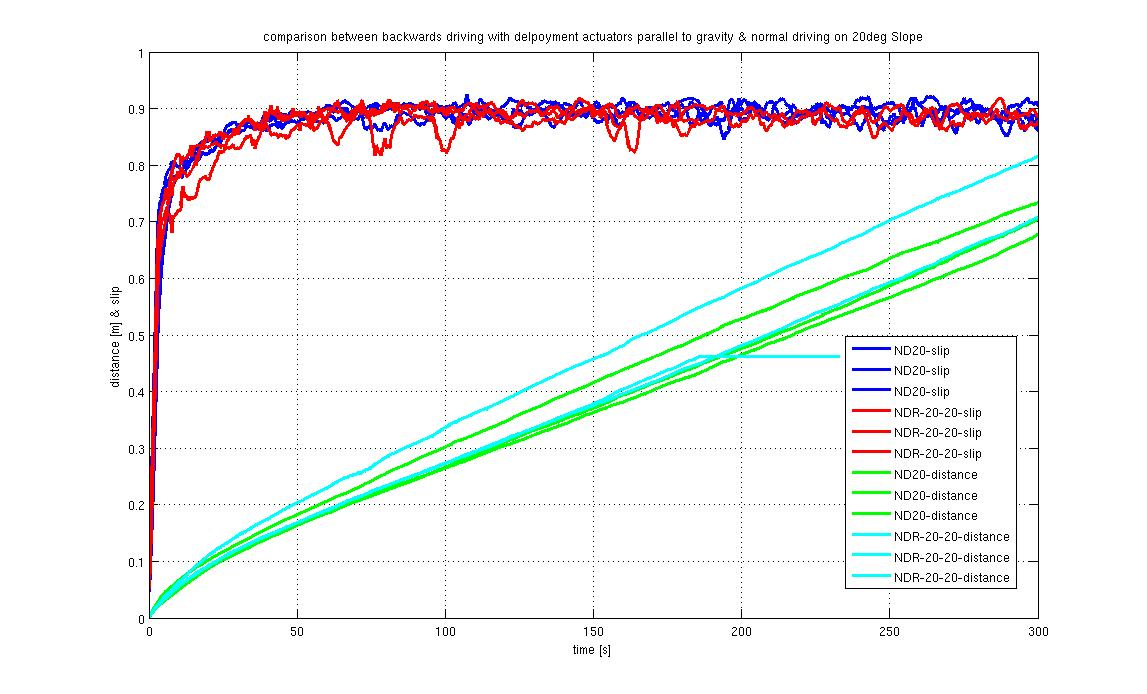
\includegraphics[width=0.9\textwidth]{ndr20d.jpg}	\caption{Comparison between
    normal driving and reverse driving with gravity aligned legs on a 20$^{\circ}$ Slope}
    \label{fig:ndr20d}
\end{figure}

%================================================================
%================================================================
\subsection{Egress Manoeuvres} The objective of this test is to find out where
wheel walking components can support the egress, one of the most challenging
manoeuvres during the lifetime of a rover. To imitate these egress conditions,
the Planetary Robotics Testbed has an adjustable egress platform.


\subsubsection{Setup and environment} The rover egress platform as shown in
pictures \ref{fig:egress29}\&\ref{fig:egress34} has two egress directions with
different slope lengths and is adjustable in its height. Thereby the egress
angle can be set. It is also adjustable to the track width of the rover. The
slopes are covered with a sticky rubber to provide sufficient traction. The
following tests had a step of 8 cm height at the end of both planks to simulate
a worst case landing in a rocky environment.  Due to the lack of any designed
flexibility in ExoTeR, the floor is prepared with foam covered by carpet to
simulate flexible wheels. 
\begin{figure}[h]
    \centering
    \subfigure{
    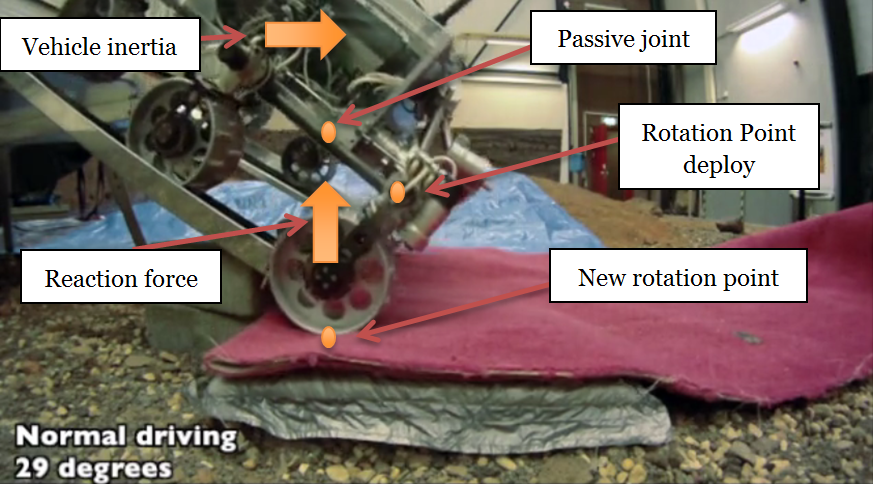
\includegraphics[width=0.9\textwidth]{egress29com.png}	}
    \subfigure{
        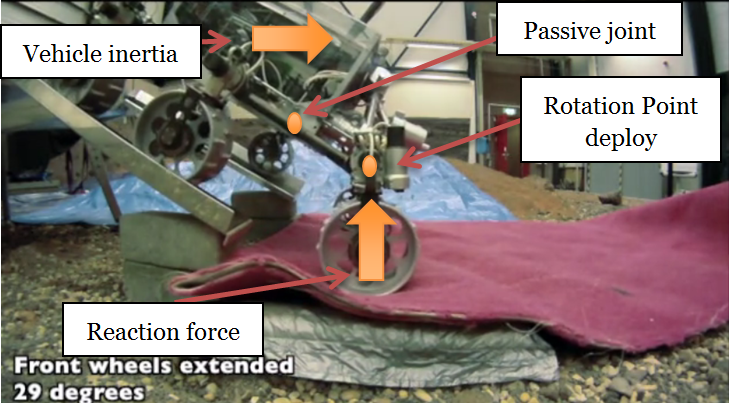
\includegraphics[width=0.9\textwidth]{egress29ext.png}	}
        \caption{Comparison between egressing in normal configuration (top) and
        34$^{\circ}$ forward shifted front wheels (bottom) on a 29$^{\circ}$
        egress slope with a step at the end} \label{fig:egress29com}
\end{figure}


Figure\ref{fig:egress29com} describes the concept behind this test. The
forward shifting of the front axis should increase the stability of the
whole system due to a bigger horizontal distance between the contact point
on the ground and the CoM. That way the angle at which it tips over is
increased. Second, due to the passive bogie, the maximum angle of egress is
limited to the angle in which the contact point on the ground falls behind
the pivot point of the bogie using their horizontal coordinate. After this
point, the two center wheels would lift off and destabilize the system even
further. In addition, the deployment actuator has to withstand very high
holding torques, both during driving and at the final impact on the ground.
Figure\ref{fig:egress29com}(bottom) has its front axle shifted by
34$^\circ$. The 34 herein is the optimized angle for the 29$^\circ$ slope
plus the 8 cm drop. 



\subsubsection{Tests}
%first the procedure

At the beginning of the test procedure, the rover is on the egress platform and
drives down with a commanded velocity of 1~\unit{cm/s}. A safety robe is
attached to its back and is hand held without tension. 

\begin{figure}[h!] \centering
    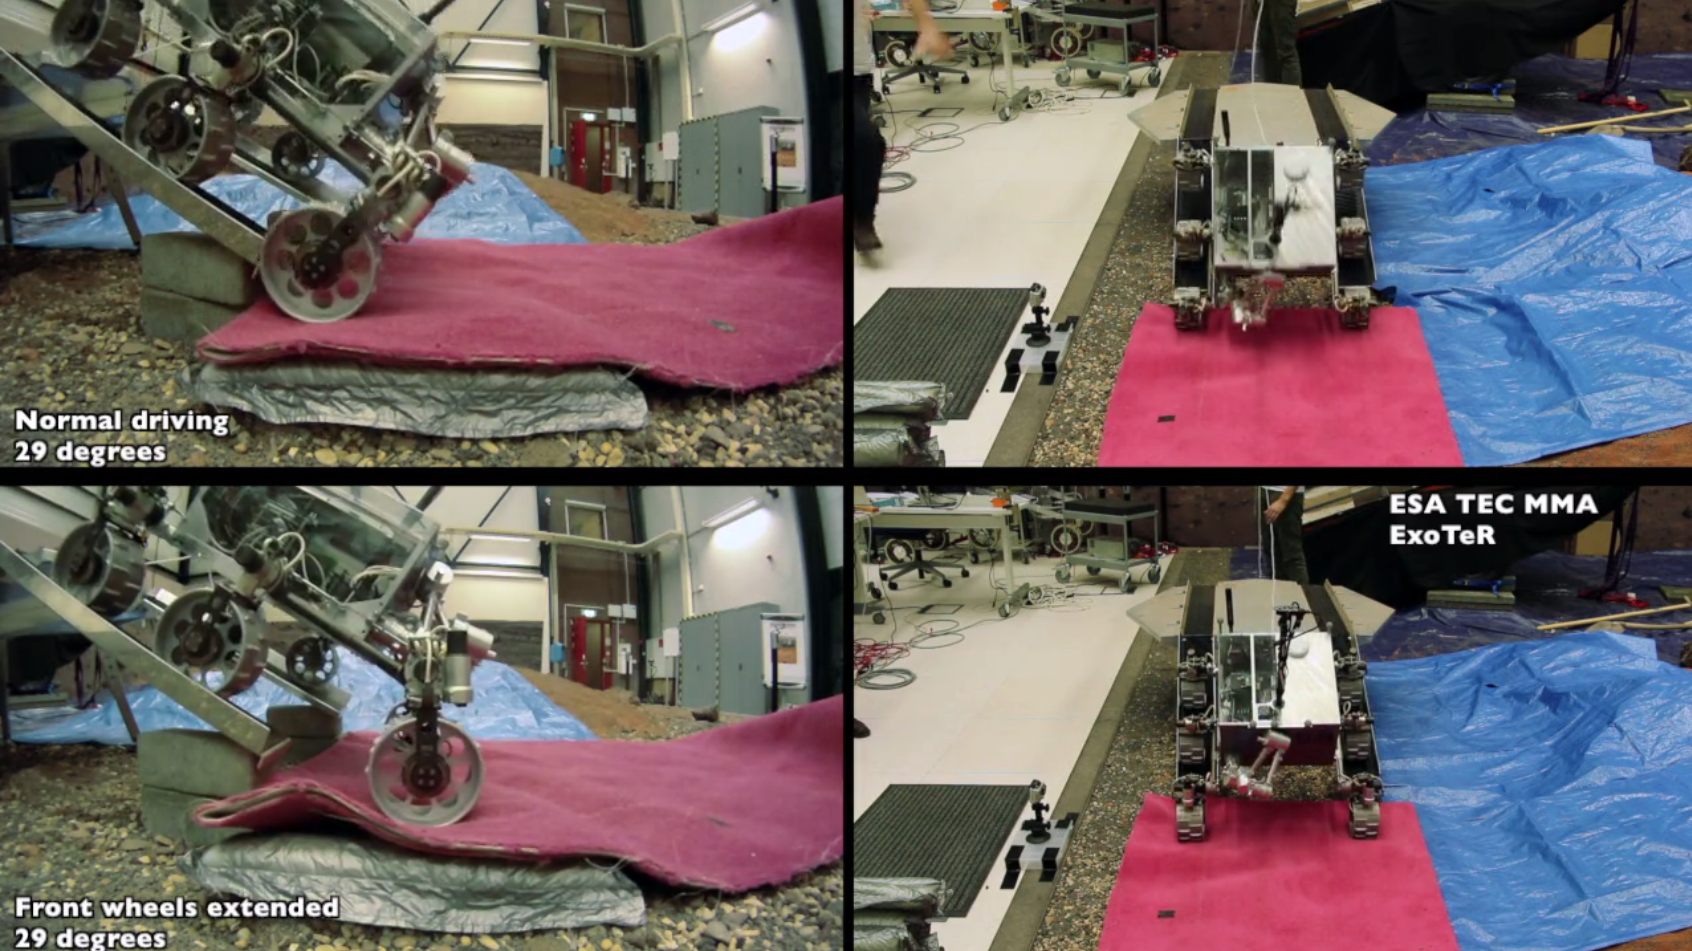
\includegraphics[width=0.9\textwidth]{egress29.png}	\caption{Comparison
    between egressing in normal configuration (top) and 34$^{\circ}$ forward
    shifted front wheels (bottom) on a 29$^{\circ}$ egress} \label{fig:egress29}
\end{figure}

\begin{figure}[h!] \centering
    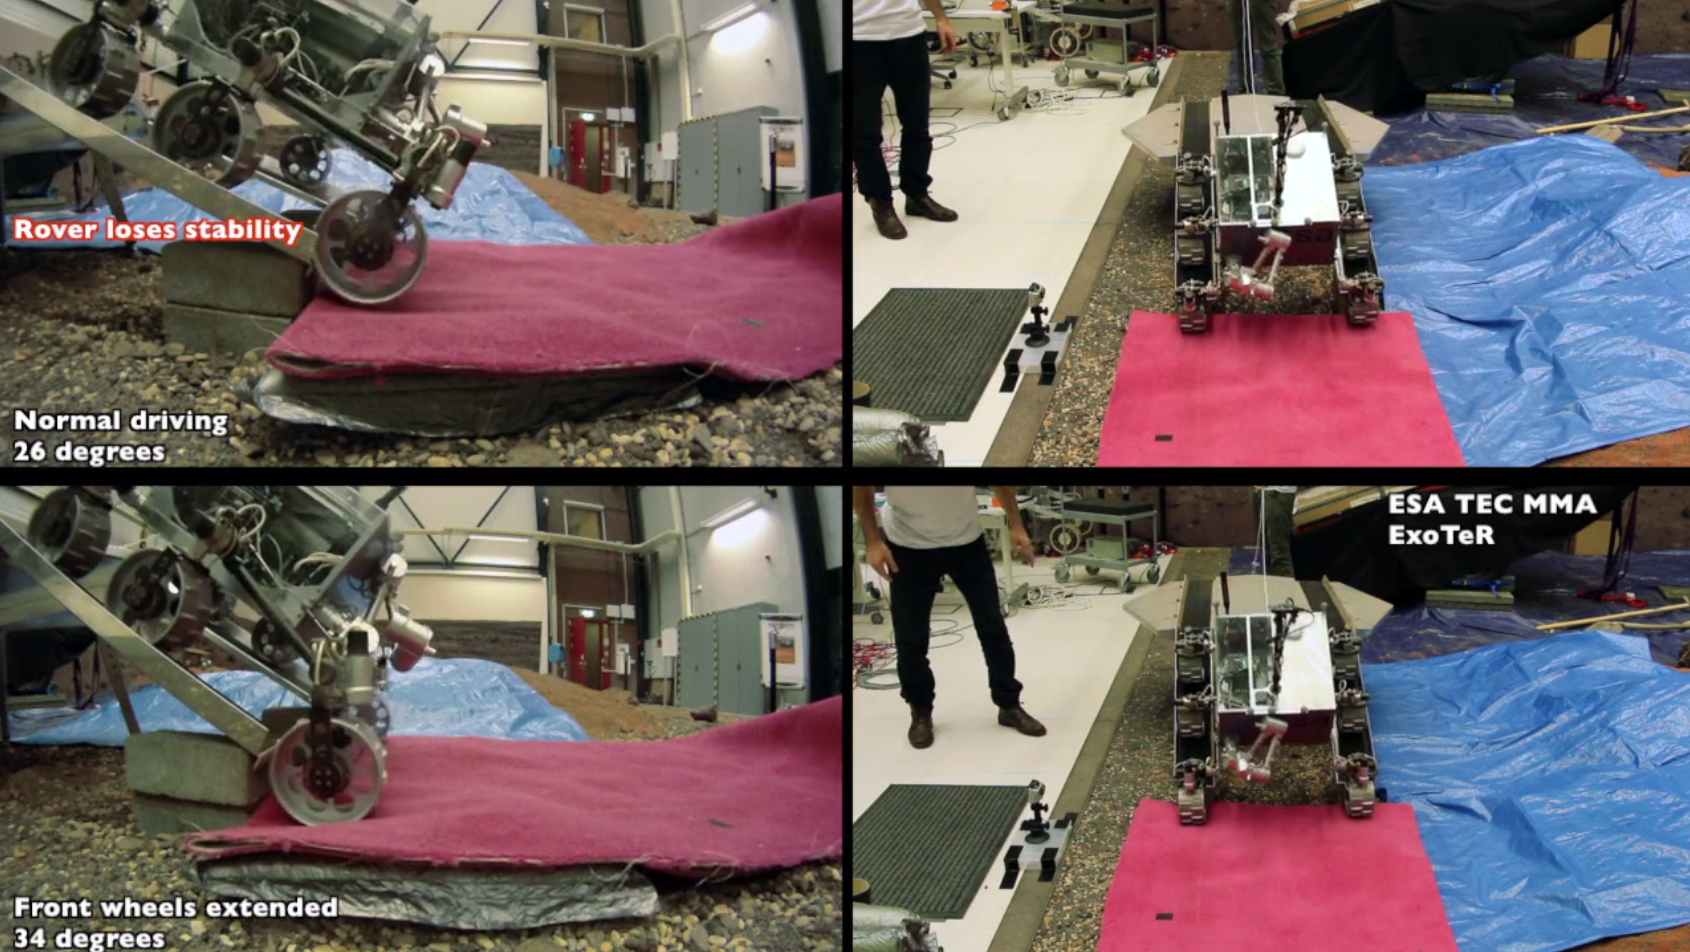
\includegraphics[width=0.9\textwidth]{egress34.png}	\caption{Comparison
    between egressing in normal configuration (top)  on a 26$^{\circ}$slope
    versus a 39$^{\circ}$ forward shifted front wheels (bottom) on a 34$^{\circ}$
    egress slope}
    \label{fig:egress34}
\end{figure}

The tests showed how the dynamic stability of the rover is increased when using
the walking mechanisms to angle the front wheel forward and verified the stated
thesis.  In standard egress manoeuvring, the rover already loses stability
(close to capsize/fall) at the slope of 26$^\circ$ (see figure
\ref{fig:egress34}(top)) and literally capsizing at the 29$^\circ$ test(see
figure \ref{fig:egress29} - top). Contrary to this, using the walking mechanisms
showed the rover going down keeping constant stability in the 34$^\circ$ slope
(see figure \ref{fig:egress34}- bottom), which is the maximum possible slope
for the current setup.

Another side observation is, that the wheel actually drops much less than the
full 8~\unit{cm} of step height. The traction of the rear four wheels is big enough to
let the front wheel pair roll down smoothly until roughly half of the wheel
diameter.

%================================================================
%================================================================
%\subsection{Results Analysis}



\section{Conclusions}

The wheel walking locomotion mode outperformed standard rolling in all the
tested scenarios demonstrating better traction in loose soil, increased
gradeability performance and improved stability limit during egress sequences.
Future rover exploration missions like ExoMars or Sample Fetching Rover could
potentially benefit from the increased locomotion capabilities of wheel walking
to reduce the chances of getting stuck in loose soil, to enable safe egress
operations or to simply allow a faster or more effective navigation by reducing
the ground track to straight distance ratio.

\section{Future Work}

Following the results of these first experiments, the Authors have decided to
continue this research path and has planned further tests to get more
experimental data and increase the confidence on the performance of wheel
walking.  Future tests will focus on slope tests to better assess the
gradeability of different wheel walking gaits in several types of soil.  The
next testing campaign is planned for March 2015 in the Robotics Mechanics
Centre (RMC) of DLR Oberpfaffenhofen.


\vspace{-3 mm}

%%%%%%%%%%%%%%%%%%%%%%%%%%%%%%%%%%%%%%%%%%%%%%%%%%%%%%%%%%%%%%%%%%%%%%%%%%%%%%%%
% \footnotesize
\bibliographystyle{aa}
\bibliography{references}

% \end{small}
\end{document}
